\begin{frame}
\frametitle{Renderizzare Un Triangolo: Demo}
\begin{figure}[ht]
    \centering
    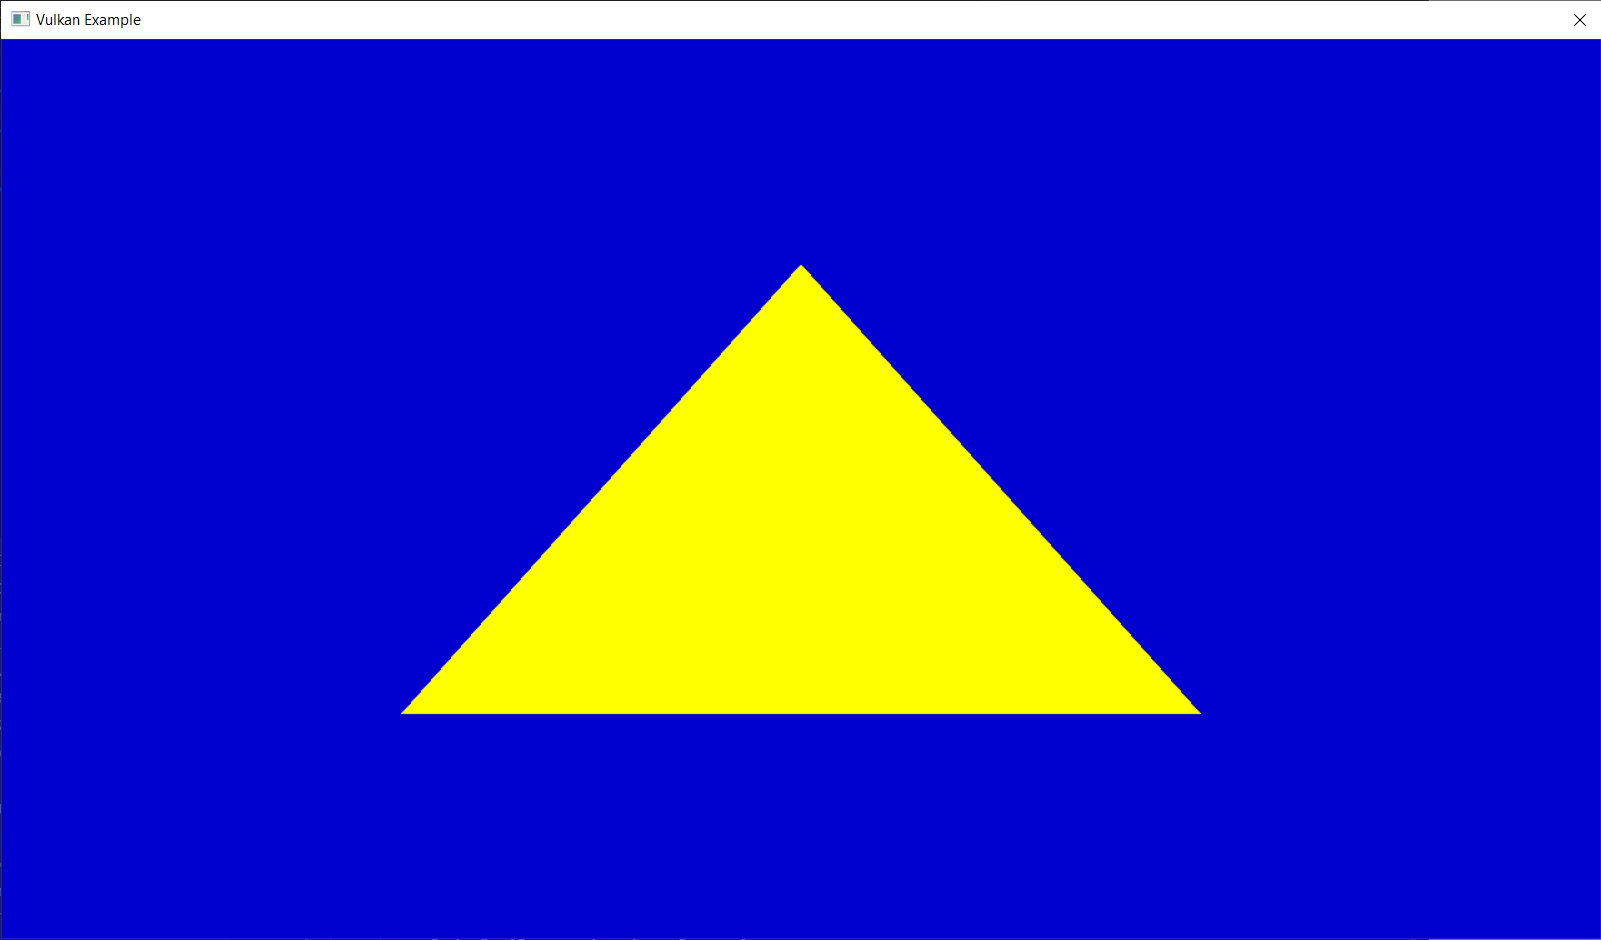
\includegraphics[scale=0.25]{images/SlidesTriangle/Triangle.png}
\end{figure}
\end{frame}

\begin{frame}
\frametitle{Renderizzare Un Triangolo}
\begin{itemize}
\item Creiamo un pipeline state object
\item Un pipeline state object descrive l'intero stato della pipeline grafica
\item Shader: programmi eseguiti dalla GPU
\item In particolare vertex shader e un fragment shader
\item La pipeline grafica riceve come input una sequenza di vertici
\item La pipeline grafica esegue il vertex shader per ogni vertice
\item Il vertex shader genera della geometria
\item La pipeline grafica esegue il fragment shader per ogni pixel coperto dalla geometria
\end{itemize}
\end{frame}
